\documentclass[12pt]{article}
\edef\restoreparindent{\parindent=\the\parindent\relax}
\usepackage{parskip}
\restoreparindent
\usepackage{german}
\usepackage{textcomp}
\usepackage{amsmath}
\usepackage{graphicx}
\usepackage{float}
\usepackage{subfigure}
\usepackage{xcolor}

\usepackage[unicode]{hyperref}
\graphicspath{ {./img/} }

\hypersetup{
  colorlinks = true,
  linkcolor = black,
  linkbordercolor = gray,
  pdfborderstyle={/S/U/W 1},
  urlcolor = blue,
  urlbordercolor = blue
}

\newcommand*{\fullref}[1]{\hyperref[{#1}]{\ref{#1} \nameref{#1}}}   % zeigt die Nummer UND den Namen an


\begin{document}

  \begin{titlepage}

    \begin{center}
      \Huge
  
      HTW-Dresden
  
      Allgemeine Informatik
  
      \bigskip
  
      \LARGE
  
      \vfill
  
      \huge
  
      \textbf{LoRaWAN Wetterstation SEN-15901}
  
      \LARGE
  
      \vfill
  
      Projektseminar\\
      Wintersemester 21/22
  
      \bigskip
  
    \end{center}
  
    \vfill
  
    \Large

  
    \vspace*{2\bigskipamount}
  
    \centering

    \begingroup
      \setlength{\tabcolsep}{12pt}
      \begin{tabular}{lll}
        Name:     & Reitz   & Rezaii-Djafari\\[2.0ex]
        Vorname:  & Lenny   & Raphael\\[2.0ex]
        s-Nummer: & s80452  & s80455
      \end{tabular}
    \endgroup
  
    \vspace*{4\bigskipamount}
  

    Tag der Einreichung: \today
  
    \vspace*{2\bigskipamount}
  
    Professor: Prof. Dr.-Ing. Jörg Vogt 
  
  \end{titlepage}

  \newpage


  \tableofcontents


  \newpage


  \section{Einleitung}
    Das Projekt wurde im Laufe des Projektseminars 2021 von Lenny Reitz und Raphael Rezaii-Djafari unter der Führung von
    Professor Jörg Vogt an der HTW Dresden entwickelt.



    \subsection{Die Übertragungstechnik: LoRa}
      LoRa (Abkürzung für Long Range) ist eine patentierte und proprietäre drahtlose Modulationstechnik basierend auf Chirp Spread Spectrum.
      Seit seiner Veröffentlichung in 2015 durch die \href{www.semtech.com}{Semtech Corporation} hat es sich für
      IoT Geräte bewährt, die außerhalb der konventionellen Reichweiten von WLAN, Bluetooth und ZigBee operieren.

      Anders als Bluetooth und WLAN können nur geringe Datenmengen mit niedriger Bitrate gesendet werden,
      dafür aber über eine erheblich größere Reichweite bei geringem Energieverbrauch. LoRa funkt standardmäßig auf dem freien Sub-1-GHz Band,
      weshalb die nutzbaren \href{https://www.thethingsnetwork.org/docs/lorawan/frequencies-by-country/}{Frequenzen}, \href{https://www.thethingsnetwork.org/docs/lorawan/duty-cycle/}{Fair-Use-Policies}
      und Vorschriften am Einsatzort beachtet werden müssen. Für eine höhere Datenrate und keine Beschränkungen gibt es auch eine
      \href{https://www.semtech.com/products/wireless-rf/lora-24ghz}{Variante mit 2.4GHz} auf die wir nicht weiter eingehen.



    \subsection{Das Protokoll \& die Architektur: LoRaWAN}
      LoRaWAN wird Open Source von der \href{https://lora-alliance.org/}{LoRa Alliance} als Systemarchitektur und Netzwerkprotokoll
      auf der Vermittlungsschicht entwickelt.

      \subsubsection{Systemarchitektur}
        Vermaschte Netze werden genutzt um eine große Abdeckung kosteneffizient zu erzielen, allerdings steht der Stromverbrauch durch die Komplexität und das
        Weiterleiten der Pakete durch die Geräte, ab hier Endknoten genannt, im Widerspruch zur geforderten Energieeffizienz der Endknoten.
        Da LoRa ohnehin eine große Reichweite besitzt, wird eine Stern-Topologie verwendet.

        Netzwerkknoten stehen dabei nicht für ein einzelnes, sondern für
        eine beliebig große Anzahl geographisch naher Gateways. Wenn ein Endknoten Daten sendet, passiert dies durch Broadcasts.
        Alle Gateways, die das Paket erhalten haben, senden es an den Netzwerk Server, der redundante Pakete herausfiltert,
        Sicherheitschecks durchführt und schließlich das Paket an seinen Bestimmungsort weiterleitet.

        \begin{figure}[h!]
          \center
          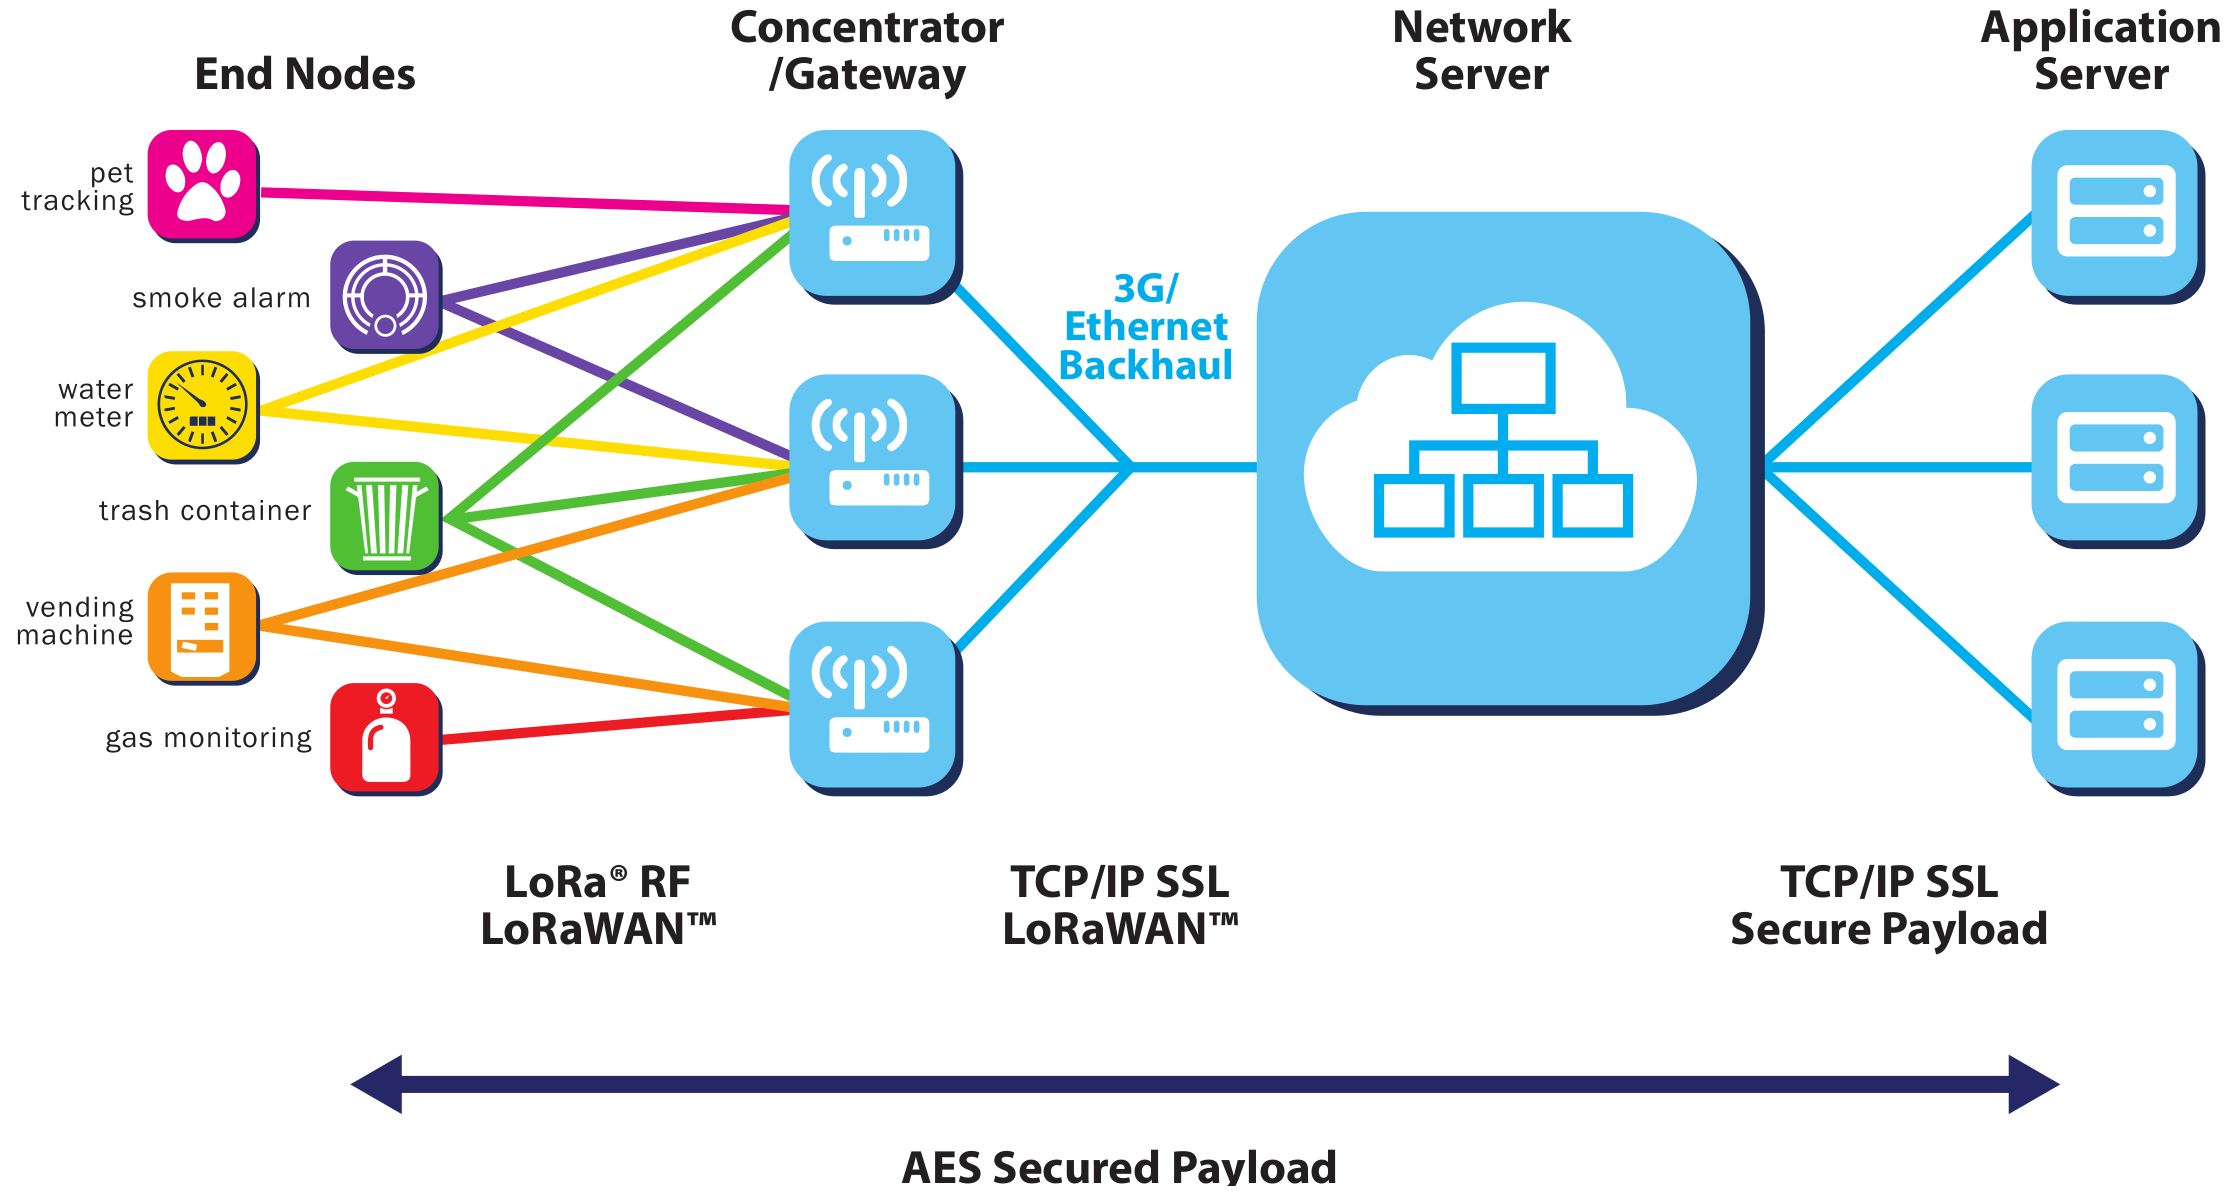
\includegraphics[scale = 0.17]{LoRaWAN_Systemarchitektur.png}
          \caption{LoRaWAN Architektur\protect\footnotemark[1]}
        \end{figure}

        Dadurch verlagert sich die Komplexität von den Endknoten und Gateways auf den Netzwerk Server.
        Außerdem wird die Verfügbarkeit verbessert, wenn ein Gateway ausfällt oder ein Endknoten mobil ist, da kein Handover notwendig ist.\footnotemark[1]

        \footnotetext[1]{LoRa Alliance. (2015). A technical overview of LoRa and LoRaWAN [Ebook] (pp. 7-9). \href{https://lora-alliance.org/wp-content/uploads/2020/11/what-is-lorawan.pdf}{https://lora-alliance.org/wp-content/uploads/2020/11/what-is-lorawan.pdf}}
    

      
      \subsubsection{Geräteklassen}
        Nicht jedes IoT Gerät hat die gleichen Anforderungen. Generell gilt, dass die Kommunikation bidirektional, asynchron und verschlüsselt erfolgt, wobei Endknoten Daten zum Netzwerk senden
        sobald diese verfügbar sind. Der Unterschied zwischen den Klassen liegt darin, wann ein Endknoten Daten vom Netzwerk empfangen kann.

        \begin{itemize}
          \item \textbf{A: batteriebetriebene Sensoren}
          
          Ein Empfangsfenster wird nur geöffnet nachdem Daten an das Netzwerk übertragen wurden. Das Netzwerk muss Downlink Kommunikation
          für das Gerät solange bereithalten bis dieses Daten sendet. Klasse A ist am energiesparsamsten und muss von allen Geräten unterstützt werden.
          
          \item \textbf{B: batteriebetriebenes Steuergerät}
          
          Zusätzlich zu den Eigenschaften der Klasse A, öffnen Geräte der Klasse B das Empfangsfenster zu festgelegten Zeiten. Eine zeitliche Synchronisation mit dem Gateway ist erforderlich.
          
          \item \textbf{C: Steuergerät mit fester Stromversorgung}
          
          Das Empfangsfenster der Geräte der Klasse C ist permanent geöffnet. Es wird nur bei Übertragungen geschlossen.
        \end{itemize}

      

      \subsubsection{LoRaWAN Netzbetreiber} \label{subsec:LoRaWAN Netzbetreiber}
        Aufgrund der Open Source Natur von LoRaWAN gibt es die verschiedensten Netzbetreiber. Wir werden uns auf das populäre
        \href{https://www.thethingsnetwork.org/}{The Things Network / The Things Stack} (TTN) beschränken.
        Es ist frei nutzbar, allerdings gibt es neben den Frequenzrichtlinien, keine Uptime Verpflichtungen und eine \href{https://www.thethingsnetwork.org/docs/lorawan/duty-cycle/}{Fair-Use-Policy}:

        \begin{itemize}
          \item Die Uplink Airtime (Endknoten \textrightarrow{} TTN) ist auf 30 Sekunden je 24 Stunden pro Endknoten beschränkt.
          \item Es dürfen maximal 10 Downlink Nachrichten (TTN \textrightarrow{} Endknoten) je 24 Stunden pro Endknoten gesendet werden.
        \end{itemize}
        
        Für die nachfolgende \underline{\nameref{subsec:Problemstellung}} eignet sich das TTN optimal. Es sei jedoch erwähnt, dass das kommerzielle \href{https://www.thethingsindustries.com/}{The Things Industries} (TTI) mit weniger Beschränkungen und SLAs existiert.
         


    \subsection{Problemstellung} \label{subsec:Problemstellung}
        Wir haben eine analoge Wetterstation und wollen diese an das TTN anbinden.
        Dafür nutzen wir einen Arduino Uno mit LoRa-Shield.

        Die Wetterstation muss verbunden und ein Programm geschrieben werden, dass die Daten ausliest und versendet.
        Die Auflösung und Anzahl der Datensätze, sowie Übertragungsparameter, Authentifizierungsmethoden und Schlüssel
        sollen einfach konfigurierbar sein.



  \section{Übersicht}

    \subsection{Hardware}
    Folgende Hardware ist Voraussetzung für den Aufbau des Projekts.
    Ein LoRa-Gateway muss dafür in Reichweite des Arduinos sein.
    Sind bereits Gateways in unmittelbarer Reichweite, ist es nicht unbedingt erforderlich ein extra Gateway zu installieren.
    Im Sinne der Unabhängigkeit und Effizienz der Kommunikation wird jedoch empfohlen, ein eigenes Gateway einzusetzen.

      \begin{itemize}
        \item \href{https://learn.sparkfun.com/tutorials/weather-meter-hookup-guide#resources-and-going-further}{Wettermessgerät-Kit SEN-15901} (enthält Regenmesser, Anemometer, Windfahne)
        \item Arduino Uno
        \item \href{https://wiki.dragino.com/index.php?title=Lora_Shield}{Dragino Lora Shield v1.4} (für Arduino Uno)
        \item LoRa Gateway (z.B. \href{https://www.dragino.com/products/lora-lorawan-gateway/item/148-lps8.html}{Dragino LPS8})
        \item 2x \href{https://www.pollin.de/p/modular-einbaubuchse-mit-anschlusslitzen-6p6c-541843}{Modular-Einbaubuchsen mit Anschlusslitzen, 6P6C}
        \item Breadboard
        \item Jumper-Kabel
        \item 1x Widerstand (10 kOhm)
      \end{itemize}

      \begin{figure}[H]
        \centering
        \subfigure[Wetterstation SEN-15901]{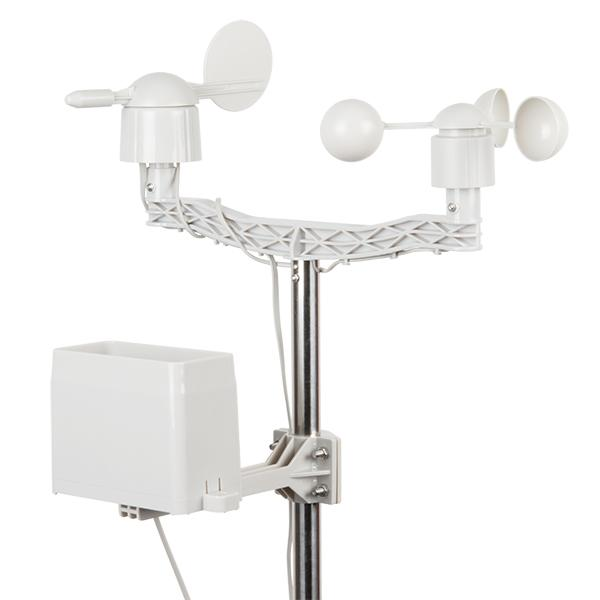
\includegraphics[scale=0.38]{Weather_Station_SEN-15901.jpg}}\qquad
        \subfigure[Dragino LoRa Gateway LPS8]{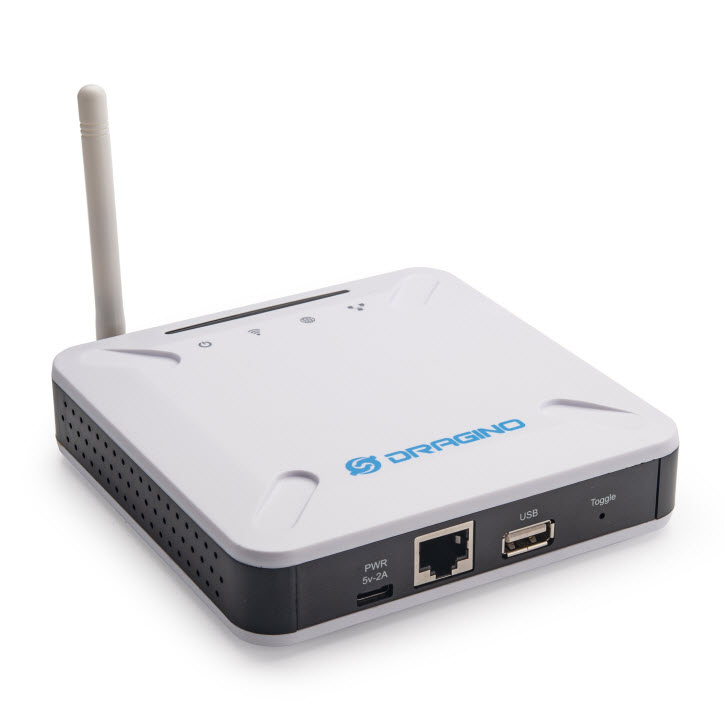
\includegraphics[scale=0.73]{Dragino_LoRa_Gateway_LPS8.jpg}}\\
        \subfigure[Dragino LoRa Shield 1.4 für Arduino]{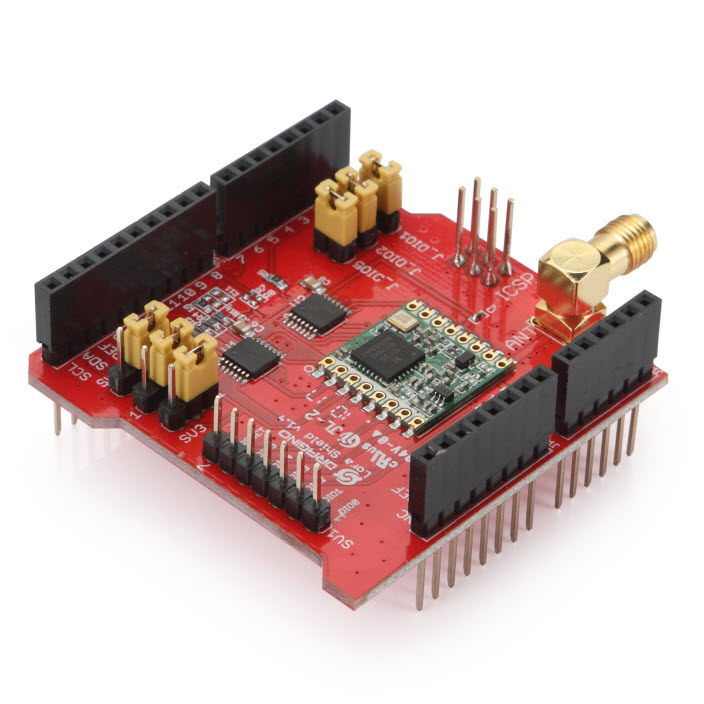
\includegraphics[scale=1]{Lora_Shield_v1.4.jpg}}\qquad
        \subfigure[RJ11 (6P6C) Einbaubuchse mit Anschlusslitzen]{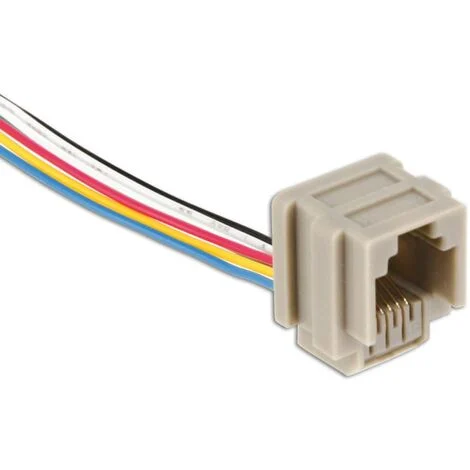
\includegraphics[scale=0.3]{RJ11_6P6C_Female_Connector.png}}
        \caption{Auswahl der benötigten Hardware \protect\footnotemark[2]}
      \end{figure}

      \footnotetext[2]{
        (a) Berrybase, Wettermessgerät-Kit für Windgeschwindigkeit, Windrichtung und Niederschlag. [image] \href{https://www.berrybase.de/sensoren-module/feuchtigkeit/wettermessger-228-t-kit-f-252-r-windgeschwindigkeit-windrichtung-und-niederschlag}{berrybase.de/sensoren-module/feuchtigkeit/wettermessger-228-t-kit-f-252-r-windgeschwindigkeit-windrichtung-und-niederschlag}.
        (b) Dragino, LPS8 Indoor LoRaWAN Gateway. [image] \href{https://www.dragino.com/products/lora-lorawan-gateway/item/148-lps8.html}{dragino.com/products/lora-lorawan-gateway/item/148-lps8.html}.
        (c) Dragino Wiki, Dragino LoRa Shield v1.4. [image] \href{https://wiki.dragino.com/index.php?title=Lora_Shield}{wiki.dragino.com/index.php?title=Lora\_Shield}.
        (d) ManoMano, Modular-Einbaubuchse mit Anschlusslitzen, 6P6C. [image] \href{https://www.manomano.de/p/modular-einbaubuchse-mit-anschlusslitzen-6p6c-13397080}{manomano.de/p/modular-einbaubuchse-mit-anschlusslitzen-6p6c-13397080}.
      }

      

    \subsection{Projektaufbau}

      \subsubsection{Wetterstation}
      Die Wetterstation hat 3 Sensoren (Regenmesser, Anemometer, Windfahne) und besitzt zwei RJ11-Stecker, über die diese ausgelesen werden können.
      Die RJ11-Stecker werden mit den beiden Einbaubuchsen verbunden, um die einzelnen Anschlüsse zuordnen zu können.
      Dann ergibt sich anhand Kabelreihenfolge bzw. -farbe folgende Belegung:

      \begin{figure}[H]
        \centering
        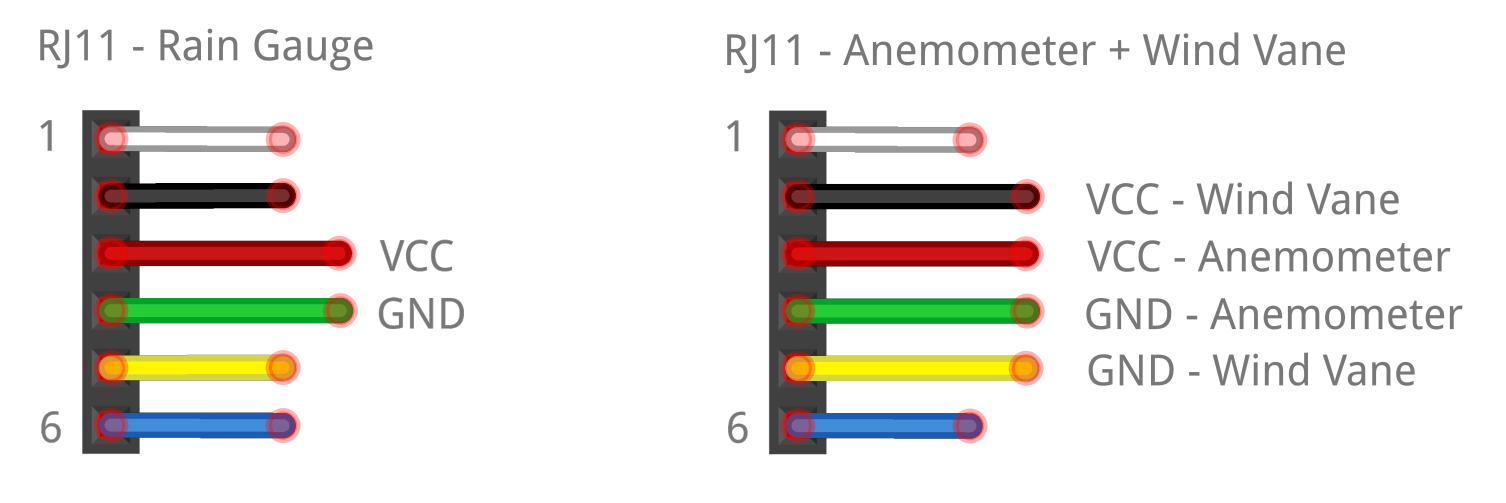
\includegraphics[scale=0.2]{Weather_Station_RJ11.png}
        \caption{Belegung der beiden RJ11-Stecker der Wetterstation}
      \end{figure}

      Ein Stecker ist demnach zum Auslesen des Regenmessers und der andere für Windfahne und Windgeschwindigkeit.



      \subsubsection{Arduino Uno (mit LoRa-Shield)}
      Der Arduino Uno bietet 6 analoge und 14 digital belegbare Pins.
      Durch den aufgesetzten LoRa-Shield werden die digitalen Pins 2 und 9 bereits belegt (siehe \href{https://wiki.dragino.com/index.php?title=File:LoRa_Shield_Pin_Mapping.png}{LoRa Shield Pin Mapping}).
      Diese beiden Pins können also zum Anschließen der Sensoren nicht mehr genutzt werden.
      Ein beispielhafter Aufbau könnte demnach so aussehen:

      \begin{figure}[H]
        \centering
        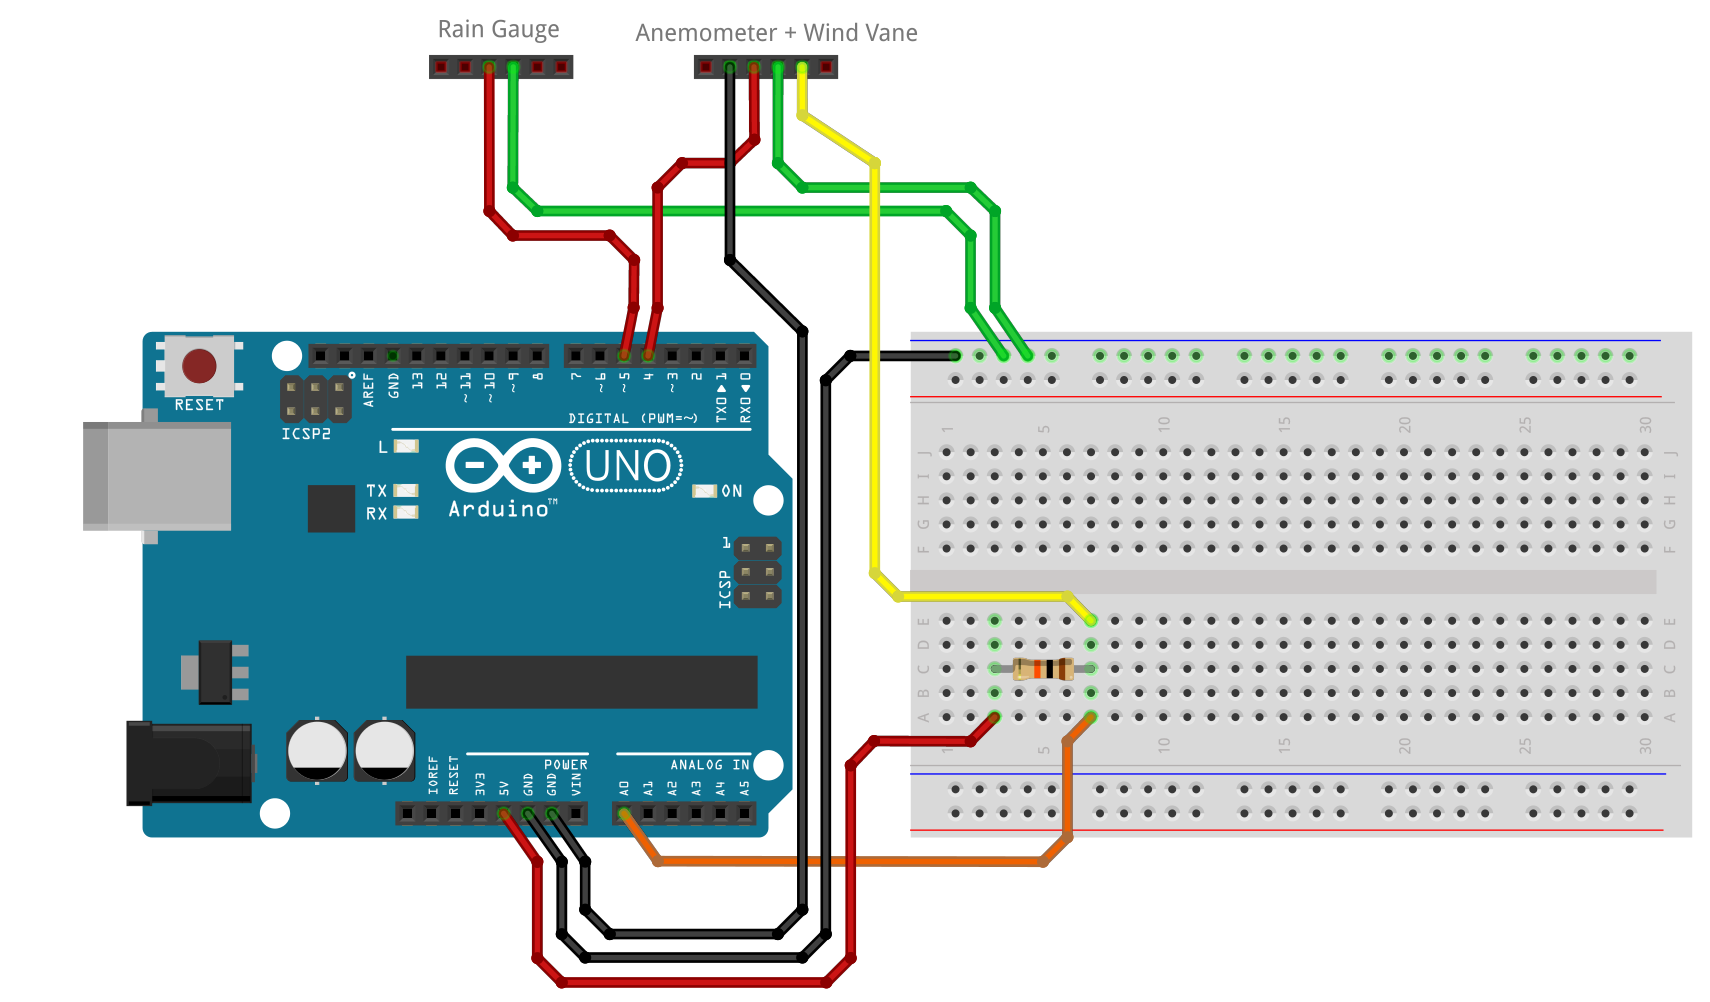
\includegraphics[scale=0.2]{Arduino_Weather_Station_Diagram.png}
        \caption{Beispielhafter Aufbau, um die Wetterstation an den Arduino anzuschließen. (Das aufgesteckte LoRa-Shield fehlt in dieser Abbildung)}
      \end{figure}

      Der Regenmesser und das Anemometer werden über die digitalen Pins 4 und 5 verbunden.
      Die Windfahne wird an den analogen Pin A0 über einen Widerstand (10 kOhm) angeschlossen.
      Einzelheiten zu der Funktionsweise der Sensoren werden in Abschnitt \underline{\ref{sensors}} erläutert.



  \section{Funktionsweise}

    \subsection{Wetterstation} \label{sensors}
    Die drei Sensoren der Wetterstation sind passive Bauelemente.
    Zum Messen muss also eine Spannung von außen (vom Arduino) angelegt werden.


    
      \subsubsection{Regenmesser}
        Der Regenmesser besteht aus einem Auffangbehälter und einem darin befindlichen einfachen Kippschalter.
        Wenn sich genügend Wasser im Behälter gesammelt hat, kippt der Schalter um und das Wasser läuft wieder aus dem Behälter heraus.
        Ein Kippvorgang entspricht einer Wassermenge von 0,2794 mm.
        Die folgende Umrechnung ergibt die Wassermenge in Milliliter bei einer Auffangfläche von 55 cm² (entspricht der Auffangfläche des Regenmessers):

        \begin{multline}
          1\,mm = 1\,l/m^2 \quad \text{(Niederschlag)} \\
          \Rightarrow 0.2794\,mm = 0.2794\,l/m^2 = 0.02794\,ml/cm^2 \\
          \Rightarrow 0.02794\,ml/cm^2 * 55\,cm^2 \approx 1.54\,ml
        \end{multline}

        Ein Kippvorgang beträgt also im Idealfall 1,54 ml.
        Mehrere Testläufe haben aber gezeigt, dass der Regenmesser mit einer relativ großen Ungenauigkeit schaltet.
        Je nach dem, wie schnell das Wasser einfließt, variiert die Messgenauigkeit stark.



      \subsubsection{Anemometer}
        Das Schalenanemometer nimmt Windgeschwindigkeiten auf, indem ein Reed-Schalter durch einen Magneten geschaltet wird.
        Je schneller sich das Anemometer dreht, umso größer wird die Schaltfrequenz.
        Eine Windgeschwindigkeit von 2.4 km/h schließt den Schalter mit einer Frequenz von 1 Hz.

        Eine Umdrehung des Anemometers entsprechen 3 Schaltvorgängen.



      \subsubsection{Windfahne}
        Die Windfahne besitzt 8 Schalter, welche jeweils mit unterschiedlich großen Widerständen verbunden sind.
        Die Schalter können einzeln oder in Paaren umgelegt werden, wodurch sich 16 mögliche Widerstandswerte und damit Himmelsrichtungen bestimmen lassen.

        \begin{figure}[H]
          \centering
          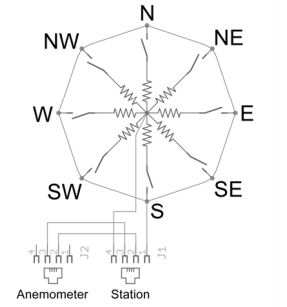
\includegraphics[scale=0.6]{Wind_Vane_Switches.jpeg}
          \caption{Aufbau der Windfahne mit den 8 verschiedenen Widerständen\protect\footnotemark[3]}
        \end{figure}

        \footnotetext[3]{
          SparkFun, The eight switches and their respective resistors internally on the wind vane. [image] \href{https://learn.sparkfun.com/tutorials/weather-meter-hookup-guide}{https://learn.sparkfun.com/tutorials/weather-meter-hookup-guide}.
        }

        Folgende Tabelle zeigt, wie die einzelnen Windrichtungen bei einer Betriebsspannung von 5 V und einem Widerstand von 10 kOhm aus der resultierenden Spannung abgelesen werden:
        
        \begin{figure}[H] \label{wind_vane_table}
          \centering
          \begin{tabular}[h]{c|c|c}
            Windrichtung & Richtung in Grad & Spannung in V \\
            \hline
            N & 0.0 & 3.84 \\
            NNE & 22.5 & 1.98 \\
            NE & 45.0 & 2.25 \\
            ENE & 67.5 & 0.41 \\
            E & 90.0 & 0.45 \\
            ESE & 112.5 & 0.32 \\
            SE & 135.0 & 0.9 \\
            SSE & 157.5 & 0.62 \\
            S & 180.0 & 1.4 \\
            SSW & 202.5 & 1.19 \\
            SW & 225.0 & 3.08 \\
            WSW & 247.5 & 2.93 \\
            W & 270.0 & 4.62 \\
            WNW & 292.5 & 4.04 \\
            NW & 315.0 & 4.33 \\
            NNW & 337.5 & 3.43 \\
          \end{tabular}
        \end{figure}



      \subsection{Arduino}
        Der Arduino Uno empfängt die Signale der Sensoren der Wetterstation über digitale und analoge Pins.
        Diese Signale müssen entsprechend verarbeitet und interpretiert werden und im Anschluss mithilfe des LoRa-Shields an das TTN übergeben werden.
        


      \subsubsection{Erfassung der Messwerte}
      Über Interrupts (siehe \href{https://github.com/HTWDD-RN/ps21-LoRa/blob/9c012bc1d41e960b6edf9e756e8948e387f28c83/src/lora_weather_station/lora_weather_station.ino#L170}{Code-Ausschnitt}), die beim Zustandswechsel der digitalen Pins ausgelöst werden, kann die Anzahl der Schaltvorgänge in einfachen Variablen (Counter) inkrementell erfasst werden.
      Der Arduino berechnet jede Sekunde einen neuen Messwert, daher werden diese Counter für Regenmesser und Anemometer jede Sekunde zurückgesetzt.
      Beide Sensoren werden außerdem zeitlich entprellt, sodass nur einmal pro Schaltvorgang inkrementiert wird.
      Das Zeitfenster, in dem die Sensoren entprellt werden, ist auf die technischen Eigenschaften der Sensoren abgestimmt, d.h. die Entprellung ist nicht so stark, dass im Zweifel Messwerte verloren gehen könnten.

      Für die Windfahne muss keine Anzahl von Schaltvorgängen ermittelt werden, da hier zu jeder Zeit der aktuelle Messwert (in Form der resultierenden Spannung) vorliegt.
      Es genügt also einmal pro Sekunde die Spannung am analogen Eingang zu messen, um die aktuelle Windrichtung bestimmen zu können.



      \subsubsection{Verarbeitung der Messwerte} \label{processing_records}
      Im nächsten Schritt werden die Messwerte für die weitere Verarbeitung unterschiedlich interpretiert.
      Allgemein wird versucht, die Datenmenge pro Messung so gering wie möglich zu halten, deshalb werden auf dem Arduino direkt keine formatierten für den Menschen lesbare Werte ausgegeben.
      Es geht alleine darum, die Messwerte für den Transport vorzubereiten.

      Die Werte für Anemometer und Regenmesser können ohne weiteres abgeschickt werden, während der Wert für die Himmelsrichtung (die abgelesene Spannung) noch komprimiert werden kann.
      Da jede Himmelsrichtung eindeutig einer Spannung zugeordnet werden kann, wird ein einfaches Array der möglichen Spannungswerte aus der Tabelle \underline{\ref{wind_vane_table}} erstellt, von dem am Ende nur die Position der Spannung im Array weitergegeben wird.
      Bei Ausgabe der Daten im TTN kann dann letztendlich mit derselben Indizierung, die zugehörige Himmelsrichtung aus einer Tabelle bestimmt werden.

      Um die Zuordnung der Spannungswerte immer gewährleisten zu können, verwendet man ein sortiertes Array der Spannungswerte (beginnend mit dem kleinsten Wert).
      Mit einem ungenau gemessenem Spannungswert kann somit einfach durch die sortierte Liste iteriert werden und an genau dem Wert im Array gestoppt werden, der dem aktuell gemessenen am nächsten kommt.
      (siehe \href{https://github.com/HTWDD-RN/ps21-LoRa/blob/9c012bc1d41e960b6edf9e756e8948e387f28c83/src/lora_weather_station/lora_weather_station.ino#L87}{Code-Ausschnitt})
      


      \subsubsection{Wetterdaten im Cache} \label{cache}
      LoRaWAN ist nicht darauf ausgerichtet, jede Sekunde neue Nachrichten zu kommunizieren.
      Es sollten immer so wenig Daten wie nötig versendet werden.
      Daher wäre es falsch jede Sekunde neue Wetterdaten zu senden.
      Der Arduino kann mehrere Messwerte zu einem Datensatz zusammenfassen und mehrere solcher Datensätze sammeln, bevor diese als Gesamtpaket versendet werden.
      Der Nutzer kann dabei selbst wählen, wie viele Messwerte zusammengefasst werden sollen (wie hoch die Auflösung sein soll) und wie viele dieser zusammengefassten Messwerte als ein Paket versendet werden sollen.
      Welche Parameter hier entscheidend sind, ist im Abschnitt \underline{\ref{sec:Konfiguration}} genauer beschrieben.

      Wie sich der Aufbau der Daten im tatsächlich versendeten Paket zusammensetzt, wird im folgenden erläutert.
      Wie im oberen Abschnitt \underline{\ref{processing_records}} beschrieben, liegen nach jeder Sekunde komprimierte Werte für die drei Sensoren vor.
      Jeder Messwert wird nun so verrechnet, dass die gewünschte zeitliche Auflösung der Werte erreicht wird.
      Folgende Werte sind dann in einem zusammengefassten Datensatz enthalten:

      \begin{enumerate}
        \item der Index der am meisten gemessenen \textbf{Windrichtung} [WV]
        \item die summierte Anzahl der Schaltvorgänge des \textbf{Regenmessers} [R]
        \item die durchschnittliche Anzahl an Schaltvorgängen des \textbf{Anemometers} [AN]
        \item die im betrachteten Zeitraum höchste Anzahl an Schaltvorgängen des \textbf{Anemometers} [M\_AN]
      \end{enumerate}

      Diese Werte eines Datensatzes werden im Anschluss auf 3 Byte verteilt (siehe \href{https://github.com/HTWDD-RN/ps21-LoRa/blob/9c012bc1d41e960b6edf9e756e8948e387f28c83/src/lora_weather_station/lora_weather_station.ino#L120}{Code-Ausschnitt}):

      \begin{figure}[H]
        \centering
        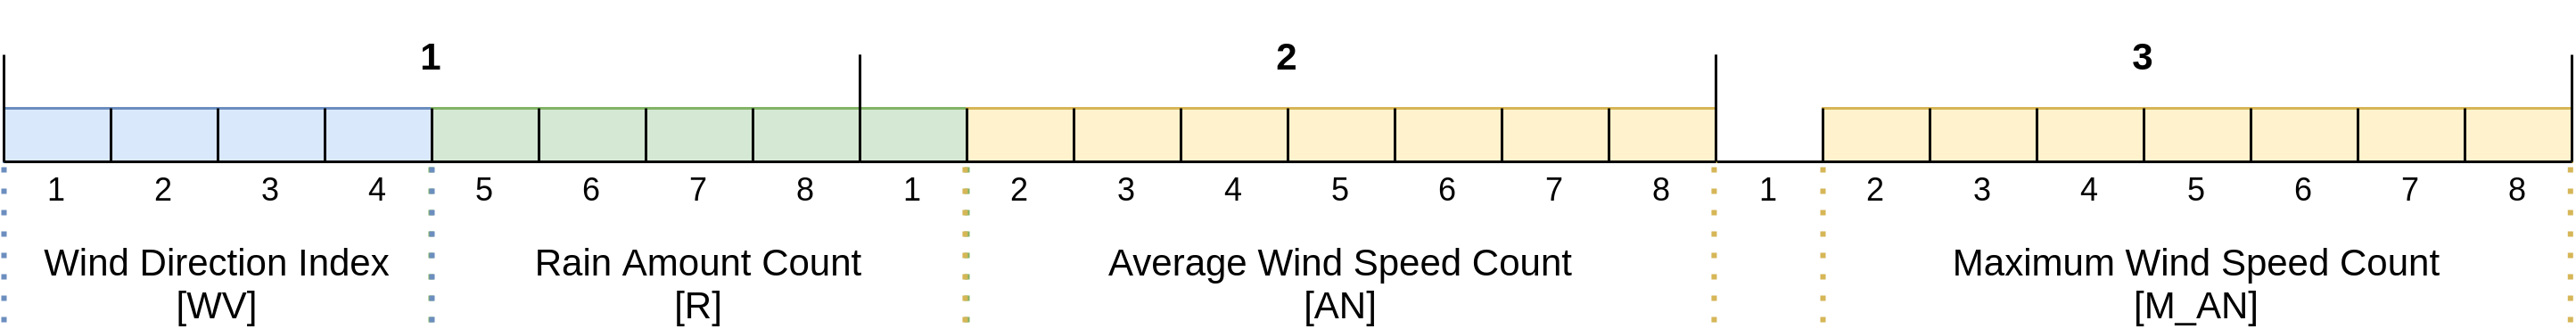
\includegraphics[scale=0.12]{Record_Byte_Representation.png}
        \caption{Aufbau eines Datensatzes}
      \end{figure}

      Die verschiedenen Wertebereiche lassen sich folgendermaßen ableiten:

      \begin{enumerate}
        \item \textbf{WV}: 4 Bit
        
        Die Windfahne misst 16 verschiedene Himmelsrichtungen.
        Übergeben wird nur der Index des sortierten Arrays der Spannungswerte (siehe \underline{\ref{processing_records}}), daher kommen hier nur Werte von 0 bis 15 zustande.
        Diese 16 Werte lassen sich exakt auf 4 Bit verteilen.

        \item \textbf{R}: 5 Bit
        
        Mit 5 Bit stehen dem Regenmesser maximal 32 Schaltvorgänge pro Zeitraum zur Verfügung.
        Durch mehrere Tests hat sich ergeben, dass der Regenmesser innerhalb von 10 Sekunden maximal 27 Schaltvorgänge auslöst.
        Das entspricht etwa einer Regenmenge von 50 mm.
        Bei einer gewählten Auflösung größer als 10 Sekunden und stärkerem Regen kann mitunter kein exakter Wert mehr übermittelt werden.
        Die vorgesehene Größe von 5 Bit reicht dazu nicht aus.
        Mögliche Lösungsvorschläge für größere Zeiträume werden im Abschnitt \ref{limits} beleuchtet. %TODO: umändern

        \item \textbf{AN}: 7 Bit %TODO: 6 Bit
        
        Die durchschnittliche Windgeschwindigkeit im betrachteten Zeitraum darf maximal 128 Schaltvorgänge auslösen.
        Das entspricht einer Windgeschwindigkeit von etwa 300 km/h.
        Solche Geschwindigkeiten werden höchstens in Ausnahmefällen erreicht und sind zudem für die durchschnittliche Geschwindigkeit äußerst unwahrscheinlich.

        \item \textbf{M\_AN}: 7 Bit %TODO: 6 Bit
        
        Die maximale Windgeschwindigkeit im betrachteten Zeitraum darf maximal 128 Schaltvorgänge auslösen.
        Das entspricht ebenfalls einer Windgeschwindigkeit von etwa 300 km/h.
      \end{enumerate}

      Je nach dem, wie viele Datensätze in einem Paket versendet werden sollen, werden die Datensätze in einem Cache zwischengespeichert.
      Ist der Cache voll, werden die Daten als ein Paket versendet.
      Der Cache wird im Anschluss geleert und kann nun wieder neu befüllt werden (siehe \href{https://github.com/HTWDD-RN/ps21-LoRa/blob/9c012bc1d41e960b6edf9e756e8948e387f28c83/src/lora_weather_station/lora_weather_station.ino#L154}{Code-Ausschnitt}).



      \subsubsection{Senden der Daten ans TTN}
      Ist der Cache voll, gibt der Arduino dem LoRa-Shield über die verwendete LMIC-Library die Anweisung alle Daten im Cache zu versenden.
      Die Art und Weise, wie die Daten über LoRa versendet werden sollen, kann der Nutzer selbst bestimmen und wird im Abschnitt \underline{\ref{sec:Konfiguration}} erklärt. %TODO: Verlinkung


    \subsection{TTN}
      Wie schon in \underline{\fullref{subsec:LoRaWAN Netzbetreiber}} genannt, nutzen wir das The Things Network.
      Zur Verwaltung der Applications (Verbund von Endknoten) und Gateways gibt es die Console.

      In dieser lassen sich Applications und Gateways erstellen, aktuelle Daten anzeigen und Einstellungen konfigurieren.
      Besonders für Endknoten interessant sind der Payload Formatter, Integrations und ADR.


      \subsubsection{Payload Formatter}          
        In diesem lassen sich Uplink und Downlink Nachrichten umwandeln.
        Bei der Übertragung über LoRa sollte die Payload stets so klein wie möglich sein, weshalb jedes versendete Bit genutzt werden sollte
        (siehe dazu auch \href{https://www.thethingsnetwork.org/docs/devices/bytes/}{Working with Bytes}).
        Damit TTN die Payload (definiert in \underline{\ref{cache}}) interpretieren kann, müssen wir einen Payload Formatter setzen,
        wie in \underline{\ref{subsec:Payload Formatter setzen}} beschrieben.
        


      \subsubsection{Integrations}
        Hier gibt es die Möglichkeit Trigger zu erstellen, die Daten verarbeiten und weiterleiten
        (bspw. Webhooks oder Storage Integrations für Up- und Downlink Nachrichten).
        Für eine Auflistung siehe \href{https://www.thethingsnetwork.org/docs/applications-and-integrations/}{Applications \& Integrations}.



      \subsubsection{Adaptive Data Rate - ADR}   
        \href{https://www.thethingsnetwork.org/docs/lorawan/adaptive-data-rate/}{ADR} ist ein Mechanismus für Endknoten
        der Spreading Factor, Daten-\\übertragungsrate und Sendeleistung optimiert. Dafür werden die letzten 20 Uplink Nachrichten analysiert.
        Es ist standardmäßig für jeden Endknoten aktiviert, sollte für mobile Endknoten jedoch deaktiviert werden (siehe\\\underline{\fullref{subsec:ADR deaktivieren}}).



    \subsection{Authentifizierungsmethoden} \label{subsec:Authentifizierungsmethoden}
      Um einen Endknoten im TTN zu authentifizieren, gibt es zwei Möglichkeiten. Beim Anlegen des Endknotens in der TTN Console muss entweder
      OTAA oder ABP gewählt werden, wobei ersteres vorzuziehen ist.

      Einen wichtigen Aspekt spielt dabei im Bezug auf Sicherheit der Frame Counter. Mit jedem gesendeten Paket wird dieser inkrementiert
      und vom Netzwerk verifiziert, um Replay-Angriffe zu verhindern.



      \subsubsection{Over-the-Air Activation - OTAA}
        Bei der bevorzugten Variante OTAA wird ein Join-Verfahren beim Einschalten des Endknotens initialisiert,
        wobei Identifikationsinformationen (inklusive Frame Counter) und Schlüssel ausgetauscht werden. Ebenso werden die verfügbaren Frequenzen und
        der optimale Spreading Factor ermittelt.

        \textit{Anmerkung:} Um Replay-Angriffe des Join-Verfahrens zu verhindern, wird eine DevNonce vom Endknoten erstellt.
        Im Optimalfall speichert der Endknoten diese persistent und sendet jedesmal eine noch nicht genutzte Nonce. Der Arduino besitzt jdedoch keinen persistenten Speicher und kann die
        bereits genutzten DevNonce nicht einsehen. In neueren MAC Versionen muss eine Nonce jeweils größer als die
        vorige sein, siehe \href{https://www.thethingsnetwork.org/forum/t/devnonce-is-too-small-what-to-do/46330}{DevNonce is too small}.
        Daher nutzen wir eine ältere MAC Version bei der der Server nur prüft ob die DevNonce bereits verwendet wurde.

        Dennoch kann es im unwahrscheinlichen Fall vorkommen, dass der Arduino zweimal die gleiche DevNonce erstellt.
        In diesem Fall verweigert das TTN die Verbindung, ein Neustarten des Arduino sollte das Problem beheben.
        


        
      \subsubsection{Activation by Personalization - ABP}
        Bei ABP werden die vordefinierten Identifikationsinformationen, Spreading Factor und Schlüssel auf dem Gerät gespeichert.
        Falls ADR deaktiviert ist, bleibt der Spreading Factor konstant. Da es keine Join-Verfahren gibt, muss der Frame Counter,
        persistent abgespeichert werden. Der Arduino Uno besitzt aber keinen persistenten Speicher. Wenn dieser nun ausgeschaltet wird, geht der Frame
        Counter verloren und beim erneuten Einschalten werden somit alle Pakete vom TTN verworfen. 

        \textit{Anmerkung:} Der Arduino Uno besitzt ein EEPROM, welchen man nutzen könnte, um den Frame Counter zu speichern. Dieser hat jedoch eine begrenzte
        Lebensdauer von ungefähr 100000 Schreibzyklen.\footnote[2]{Egger, Alexander. Arduino und der EEPROM. Retrieved 10 February 2022, from \href{https://www.aeq-web.com/arduino-atmega-eeprom-read-write-details/}{https://www.aeq-web.com/arduino-atmega-eeprom-read-write-details/}}
        Der Versuch den Frame Counter im RAM zu behalten und nur beim Ausschalten zu speichern funktioniert nicht, da bei einem Stromausfall
        die Operation nicht durchgeführt wird. Um das zu umgehen, kann mit jedem gesendeten Paket der EEPROM beschrieben werden. Dann ist dieser nach
        spätestens 100000 Paketen nicht mehr beschreibbar, was abhängig vom Sendeinterval schnell sein kann.

        Daher empfehlen wir unbedingt OTAA zu verwenden. Soll dennoch ABP genutzt werden, so lässt sich in der TTN Console die Frame Counter Überprüfung deaktivieren,
        wie gezeigt in \underline{\fullref{subsec:ABP - Konfiguration}}, wodurch\\Replay-Angriffe nicht mehr verhindert werden.

        Weiterhin gibt es noch ein Problem mit den nutzbaren Frequenzen, siehe \underline{\fullref{subsec:ABP - Frequenzbereich}}, was aber OTAA nicht betrifft.
  
      

  \section{Konfiguration \& Verbindung der Wetterstation} \label{sec:Konfiguration}
    \textit{Anmerkung:} Es gibt auch einen Quelltext der die Daten lokal auswertet, ohne jegliche LoRa Implementationen
    (siehe \texttt{local\_weather\_station.ino}).

    Weiterhin wird in dieser Dokumentation nicht darauf eingegangen, wie ein Gateway eingerichtet wird.
    Konsultieren Sie dafür die Betriebsanleitung des Herstellers.

    \textbf{Vorbedingung:}
    \begin{enumerate}
      \item Installieren Sie die Arduino IDE und die notwendige \href{https://github.com/dragino/arduino-lmic}{Library} nach \texttt{Installation.md}
      \item Erstellen Sie einen TTN Account unter \href{www.thethingsnetwork.org}{www.thethingsnetwork.org}
      \item Navigieren Sie zur Console
      \item Wählen Sie \textless Go to applications\textgreater{}
      \item Fügen Sie durch \textless Add application\textgreater{} eine Application hinzu
      \item Wählen Sie \textless Add end device\textgreater{} und wechseln in den \textless Manually\textgreater{} Tab
      \item Frequency Plan: Europe 863-870 MHz (SF9 for RX2 - recommended)
      \item LoRaWan version: MAC V1.0.2
      \item Regional Parameters version: PHY V1.0.2 REV A
    \end{enumerate}
    
    Wie bereits in \underline{\fullref{subsec:Authentifizierungsmethoden}} erläutert, empfehlen wir OTAA gegenüber ABP.



    \subsection{OTAA - Konfiguration}
      \begin{enumerate}
        \setcounter{enumi}{9}
        \item DevEUI: Generate
        \item AppEUI: Fill with zeros
        \item AppKey: Generate
        \item \textless Register end device \textgreater{}
        \item Wechseln Sie zu \texttt{secret.template.h} und geben Sie die generierten Daten ein.
          Achten Sie ggf. auf das little-endian Format.
        \item Benennen Sie \texttt{secret.template.h} in \texttt{secret.h} um
        \item Öffnen Sie \texttt{config.h} und aktivieren Sie den OTAA Modus
        \item Wählen Sie Ihre gewünschten Datenauflösung und die Größe der Payload.
          Betrachten Sie dazu das Beispiel und verifizieren Sie die Größe der Payload mit dem
          \href{https://www.thethingsnetwork.org/airtime-calculator}{LoRaWAN airtime calculator}.
        \item Prüfen Sie, dass die \href{https://www.thethingsnetwork.org/docs/lorawan/duty-cycle/}{Fair-Use-Policy} nicht verletzt wird
        \item Beachten Sie, dass bei OTAA der Spreading Factor automatisch gesetzt wird.
          Wählen Sie am besten Werte die mit SF12 noch unter die Fair-Use-Policy fallen.
        \item Falls gewünscht, können Sie \underline{\nameref{subsec:ADR deaktivieren}}.
        \item Installieren Sie das Programm auf dem Arduino Uno.
        \item Machen Sie weiter mit \underline{\nameref{subsec:Payload Formatter setzen}}.
      \end{enumerate}



    \subsection{ABP - Konfiguration} \label{subsec:ABP - Konfiguration}
      \begin{enumerate}
        \setcounter{enumi}{9}
        \item \textless Show advanced activation, LoRaWAN class and cluster settings \textgreater{}
        \item Activation mode: ABP
        \item DevEUI: Generate
        \item Device address: Generate
        \item AppSKey: Generate
        \item NwkSKey: Generate
        \item \textless Register end device \textgreater{}
        \item Nachfolgend deaktivieren Sie den Frame Counter, siehe Problematik in \underline{\fullref{subsec:Authentifizierungsmethoden}}.
        \item Wechseln Sie in den \textless General settings\textgreater{} Tab
        \item Wählen Sie bei Network layer \textless Expand\textgreater{}
        \item Wählen Sie unten \textless Advanced MAC settings\textgreater{}
        \item Setzen Sie das Häkchen in \textless Resets frame counters\textgreater{}
        \item Falls gewünscht, entfernen Sie das Häkchen bei \textless Use adaptive data rate (ADR)\textgreater{}
        \item \textless Save changes\textgreater{}
        \item Wechseln Sie zu \texttt{secret.template.h} und geben Sie die generierten Daten ein.
        \item Benennen Sie \texttt{secret.template.h} in \texttt{secret.h} um
        \item Öffnen Sie \texttt{config.h} und aktivieren Sie den ABP Modus
        \item Wählen Sie Ihre gewünschten Datenauflösung und die Größe der Payload.
          Betrachten Sie dazu das Beispiel und verifizieren Sie die Größe der Payload mit dem
          \href{https://www.thethingsnetwork.org/airtime-calculator}{LoRaWAN airtime calculator}.
        \item Prüfen Sie, dass die \href{https://www.thethingsnetwork.org/docs/lorawan/duty-cycle/}{Fair-Use-Policy} nicht verletzt wird.
        \item Falls gewünscht, können Sie \underline{\nameref{subsec:ADR deaktivieren}}.
        \item Installieren Sie das Programm auf dem Arduino Uno.
        \item Machen Sie weiter mit \underline{\nameref{subsec:Payload Formatter setzen}}.
      \end{enumerate}



    \subsection{ADR deaktivieren} \label{subsec:ADR deaktivieren}
      \begin{enumerate}
        \item Wechseln Sie in den \textless General settings\textgreater{} Tab im TTN
        \item Wählen Sie bei Network layer \textless Expand\textgreater{}
        \item Wählen Sie unten \textless Advanced MAC settings\textgreater{}
        \item Entfernen Sie das Häkchen in \textless Use adaptive data rate (ADR)\textgreater{}
        \item \textless Save changes\textgreater{}
      \end{enumerate}


    
    \subsection{Payload Formatter setzen} \label{subsec:Payload Formatter setzen}
    \begin{enumerate}
      \item Wählen Sie den \textless Payload formatters\textgreater{} Tab
      \item Uplink ist standardmäßig ausgewählt
      \item Formatter type: Javascript
      \item Kopieren Sie den Javascript Code von \texttt{payload\_formatter.js} in das vorgesehene Feld
      \item \textless Save changes\textgreater{}
      \item Testen Sie den Formatter mit der Payload X %TODO: add payload
      \item Starten Sie den Arduino. Falls ein Gateway in Reichweite ist, sollten die Daten nach einiger
        Zeit im Tab \textless Live data\textgreater{} erscheinen
    \end{enumerate}



  \section{Limitierungen}

      \subsection{ABP - Frequenzbereich} \label{subsec:ABP - Frequenzbereich}
        In Europa ist der Downlink Frequenzbereich 868.1 - 868.8 MHz.
        Die Anwendung wechselt dabei automatisch zwischen den Kanälen, um eine gleichmäßige Auslastung zu erzielen.

        Bei OTAA werden die nutzbaren Frequenzen beim Join-Verfahren vom Netzwerk übertragen.
        Weil ABP dieses nicht nutzt, müssen diese Frequenzen jedoch vordefiniert werden.

        Wenn das Programm im ABP Modus läuft, funktionieren nur die Frequenzen: 868.1, 868.3, 868.5MHz.
        Wahrscheinlich setzen wir die zusätzlichen Frequenzen nicht korrekt.
        Im \href{https://github.com/dragino/arduino-lmic/blob/f2775468e19b2c2a35557ef2f8255cffb2a783be/examples/ttn-abp/ttn-abp.ino#L180}{Codebeispiel der Library}
        wurden diese leider deaktiviert.

        Wenn wir die zusätzlichen Frequenzen hier freischalten, sendet das Gateway bei Paketen die nicht auf den 3 oben genannten Frequenzen gesendet wurden, keine Downlink Nachricht
        und quittiert dem Endknoten das Paket nicht.


        
  \section{Fazit}
    \begin{itemize}
      \item für beide sehr interessant
      \item noch nie mit Arduino gearbeitet und wenig Mikrocontroller Erfahrung
      \item auch noch nie LoRa, ins Kalte Wasser geschmissen
      \item schwierige Programmierung mit Geräten die nicht häufig in der Community zumindest TTN genutzt werden
      \item Änderung auf TTNv3 hat es auch nicht besser gemacht
      \item viele Libraries, die aber alle nicht funktioniert haben, erst über Tipp der anderen Gruppe von angepasster Dragin Library erfahren
      \item Debugging ist schwierig bis unmöglich ohne eigenes Gateway, wahrscheinlich am Sinnvollsten einen RaspberryPI dafür zu nutzen
      \item 
    \end{itemize}
    
  

\end{document}